\chapter{Evaluation}

\label{Chapter4}

\lhead{Chapter 4. \emph{Evaluation}}

\section{Description of the evaluated dataset} % (fold)
\label{eval:sec:description_of_the_evaluated_dataset}

% section description_of_the_evaluated_dataset (end)

\section{Prerequisites} % (fold)
\label{eval:sec:prerequisites}

For any of this user adaptation to have any actual use, we will need to find out whether there is actually significant variation in feature adoption between clusters; it matters little whether users exhibit differing behavior with regard to existing functionality, if this behavior yields no basis for predicting feature adoption in the future. We need an inductive bias.

An easy way of discovering whether this inductive bias is present in the user base is to simply log whether there is significant variance across the user groups in their users' adoption of new features. Thus, this question of whether the predictive bias actually exists will be included as a central part of the actual experiment itself, and be thoroughly discussed through the next sections.

% section prerequisites (end)

\section{Experimental setup} % (fold)
\label{eval:sec:experimental_setup}

\emph{Condensed version.}

The main experiment determines whether an alteration of the service affects different kinds of users differently.
More specifically, do users in clusters $C_1, \ldots, C_n$ employ function $f$ in significantly differing ways? We find out without touching a large percentage of the users, and can use the results to individually enable features for users that

We break the process into three steps, each elaborated on in~\ref{approach:sec:identifying_adaptability}, \ref{approach:sec:clustering}, and \ref{approach:sec:adaptation_component}:

\begin{enumerate}
  \item A/B test feature $f$ on a percentage of all users.
  \item Separate users into clusters $C_1, \ldots, C_n$.
  \item Analyze results: did the test results vary significantly between clusters?
\end{enumerate}

If the final answer is ``yes'', we can store our results and use them as a basis for adaptating the interface for each user.

\subsection{A/B testing features} % (fold)
\label{eval:sec:a_b_testing_features}

\emph{@TODO: Brief description of how to fit the actual testing regime into the production system.}

% subsection a_b_testing_features (end)

\subsection{User clustering} % (fold)
\label{eval:sec:clustering_of_users}

\begin{figure}[h]
  \centering
    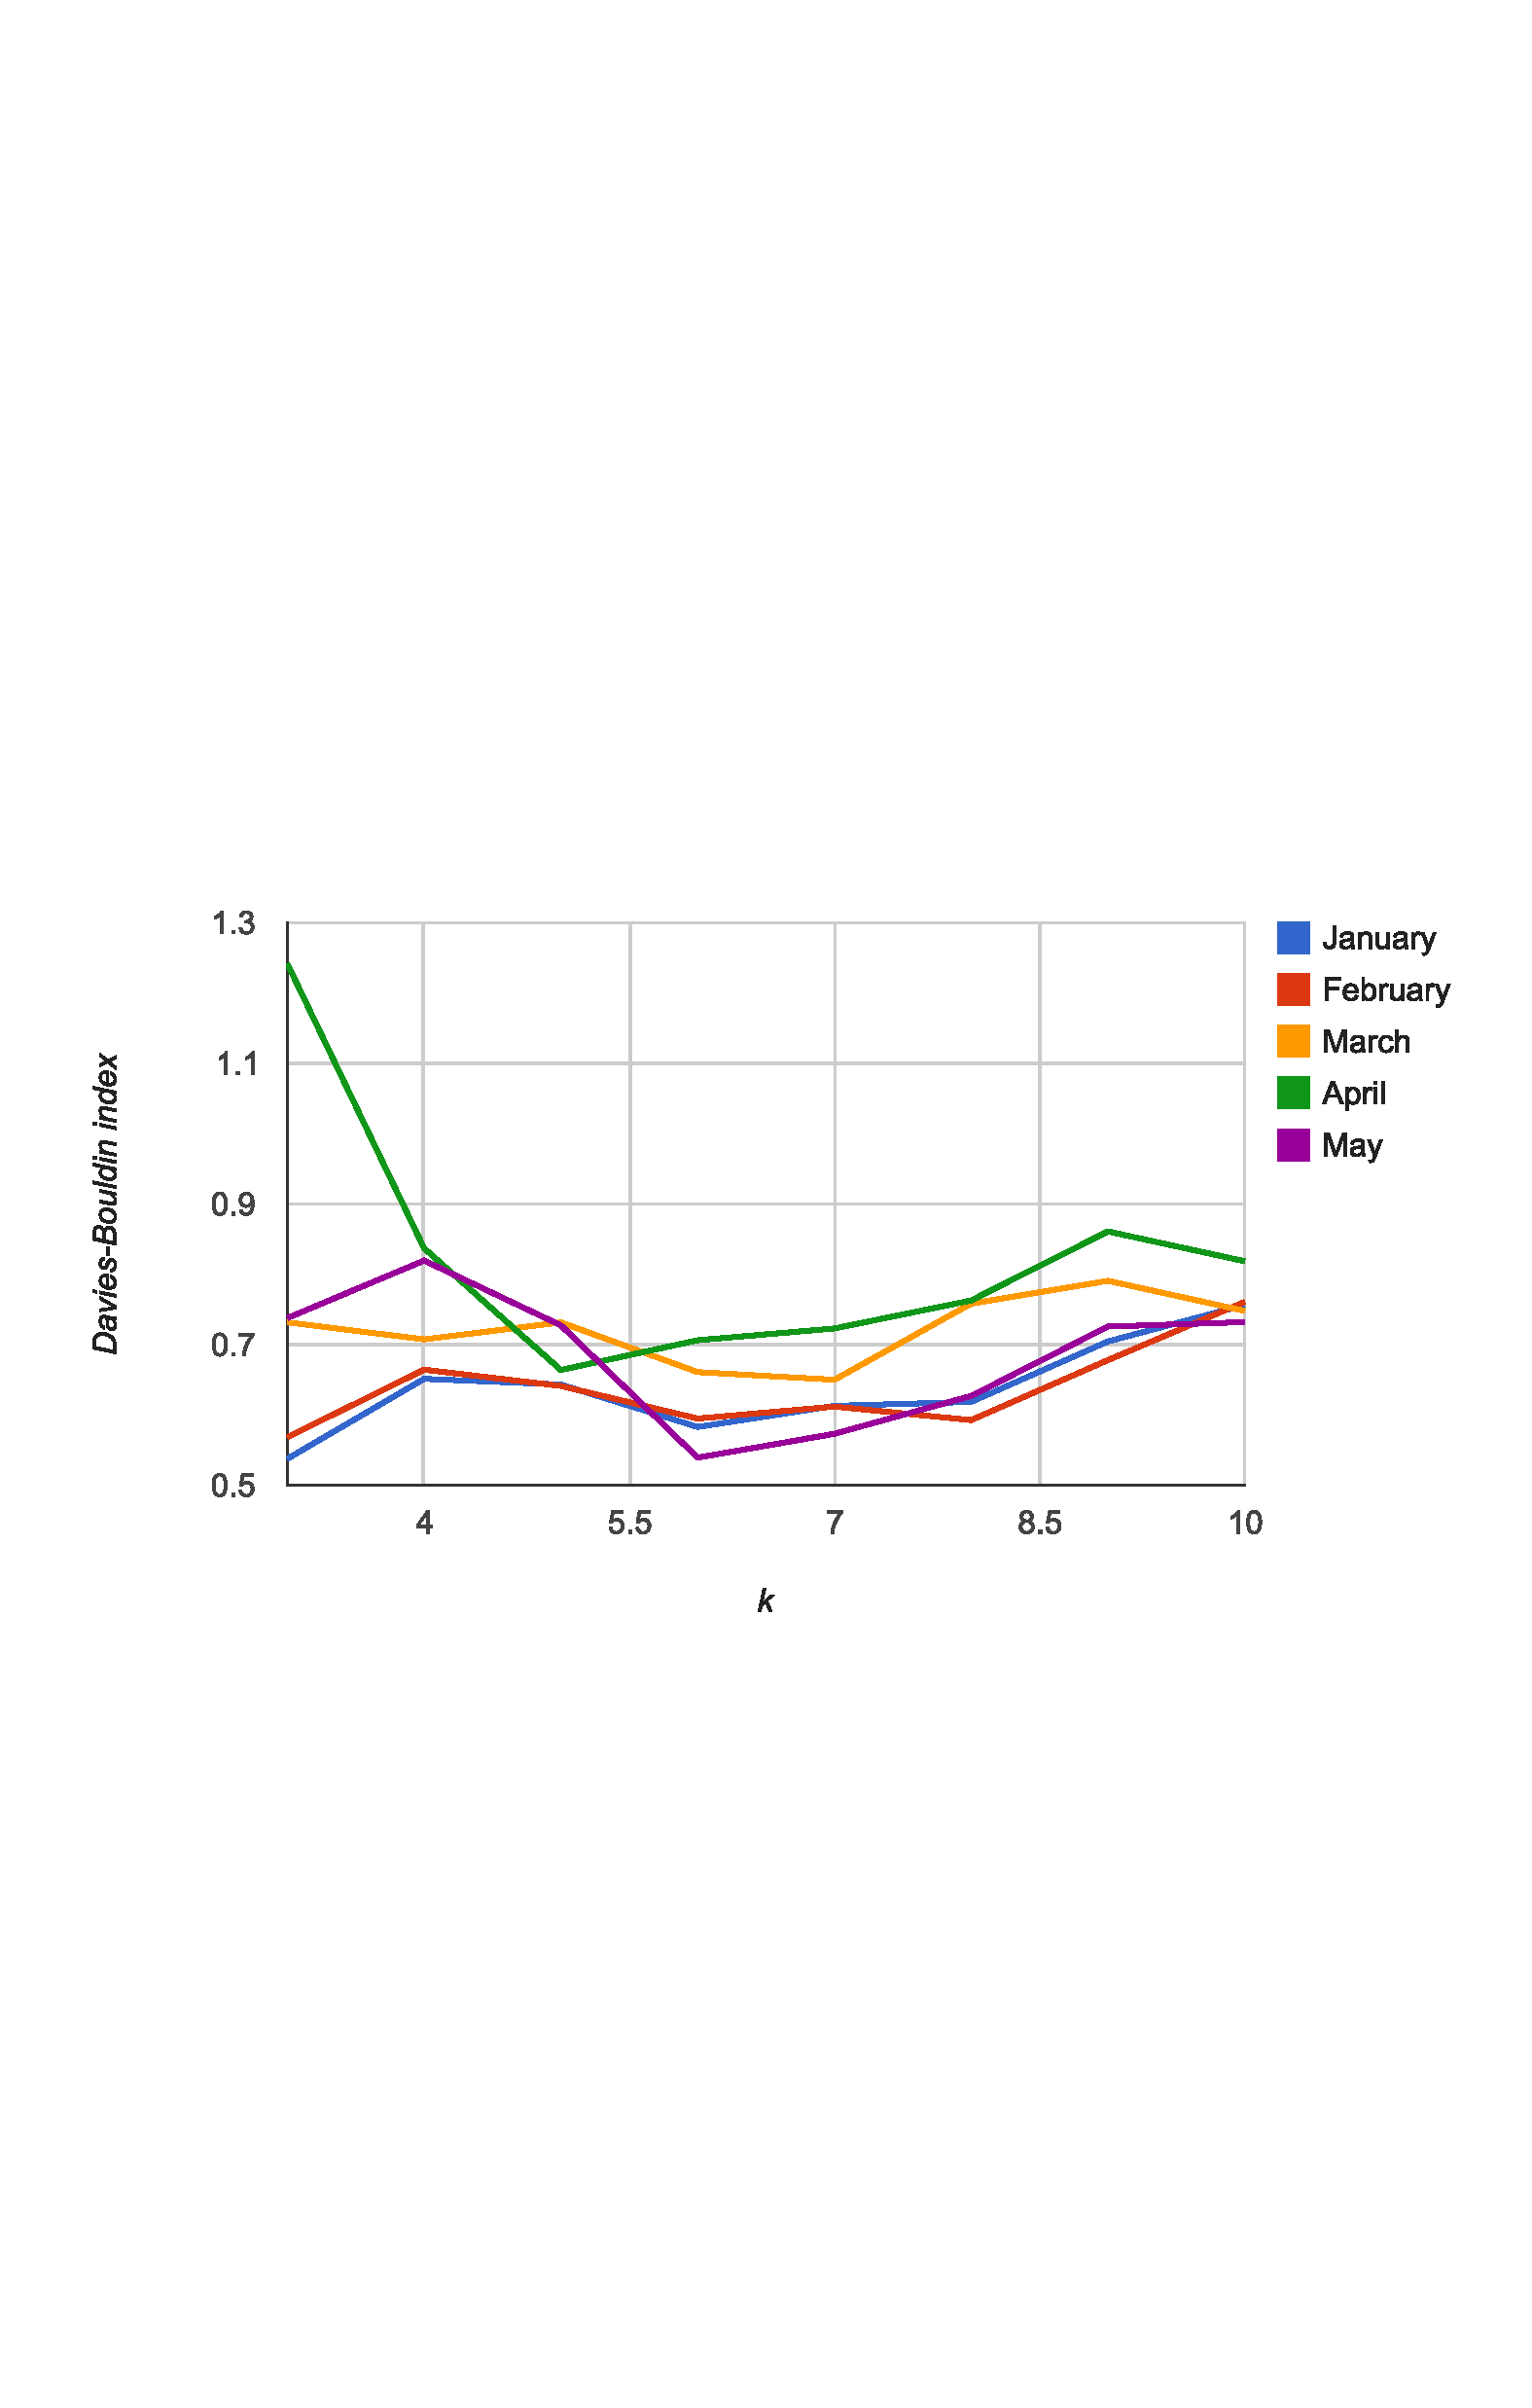
\includegraphics[width=\textwidth]{Figures/plots/k-vs-db/jan-may}
    \caption{$k$ vs. Davies-Bouldin index, for clusters with data for January to May.}
    \label{fig:k_vs_db}
\end{figure}

\emph{@TODO: Describe methods and algorithms used. What kind of results are expected?}

% subsection clustering_of_users (end)


% section experimental_setup (end)

\section{Initial clustering results}
\label{eval:sec:clustering_results}

The data used in this analysis stems from February 2014.

The following clustering results were found by choosing the best of 5 k-means runs, ``best'' being defined by their Davies-Bouldin indices (see section~\ref{approach:sub:evaluating_clusters} for a brief description of this evaluation metric). This process was performed for $k$ parameter values from 3 to 10, where $K = 8$ yielded the best result. The 2 smallest resulting clusters were omitted in the analysis due to their relatively insignificant sizes.

Data from January and March yield more or less the same results, although they are a bit less clear. This could be due to media events and holidays generating more skewed data than usual.

\begin{figure}[h]
  \centering
    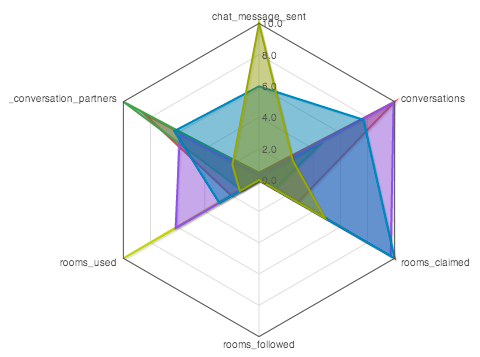
\includegraphics[width=0.8\textwidth]{Figures/clusterings/confluence-post/comp-02-feb}
    \caption{Radar chart comparing clusters generated from data for February 2014.}
    \label{fig:radar-clusters-february}
\end{figure}

The radar chart in figure~\ref{fig:radar-clusters-february} shows the centroids of 6 large clusters $C$ relative to each other.

Each dimension's centroid values $\mu_i \in \mu$ have been scaled by a factor of $\frac{10}{\max_{c \in C}{c_i}}$, to fit nicely inside the chart.

The features used in this particular clustering run are (going clockwise around the chart):

\begin{enumerate}
  \item chat messages sent
  \item conversations (2+ persons present in room)
  \item rooms claimed
  \item rooms followed
  \item unique rooms used
  \item conversation network size (ie. number of unique other users within 2 degrees of conversation separation)
\end{enumerate}

Most of these features are quantified by counting the number of relevant events logged for each user.

\subsection{The typical clusters}
\label{eval:sec:typical_clusters}

\emph{@TODO: Should this part be moved to appendix?}

To know what types of users we are dealing with through the next chapters, let's walk through the clusters discovered in the February dataset, as described above.

\begin{figure}
  \centering
  \begin{subfigure}[t]{0.45\textwidth}
    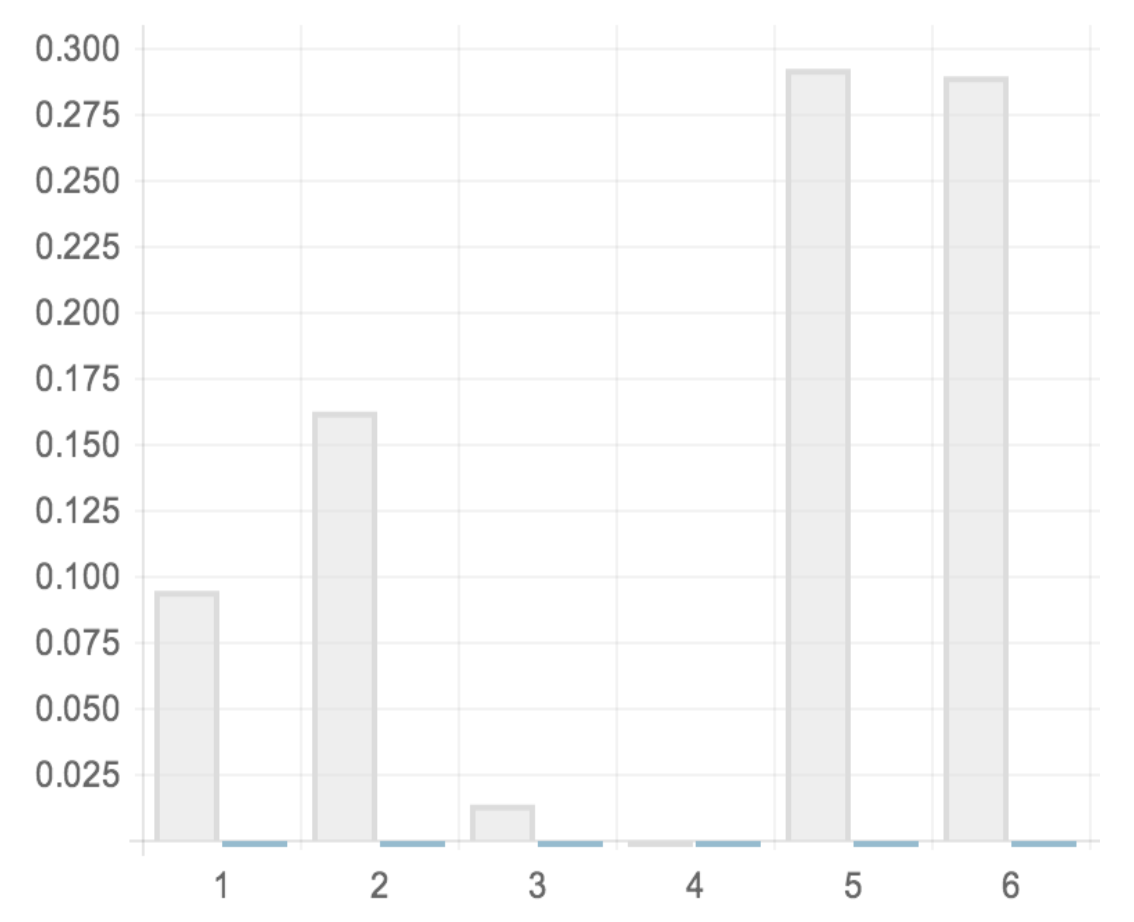
\includegraphics[width=\textwidth]{Figures/clusterings/confluence-post/cluster1-chart}
    \caption{Cluster 1: Front page hitting users}
    \label{fig:cluster1-chart}
  \end{subfigure}
  \hfill
  \begin{subfigure}[t]{0.45\textwidth}
    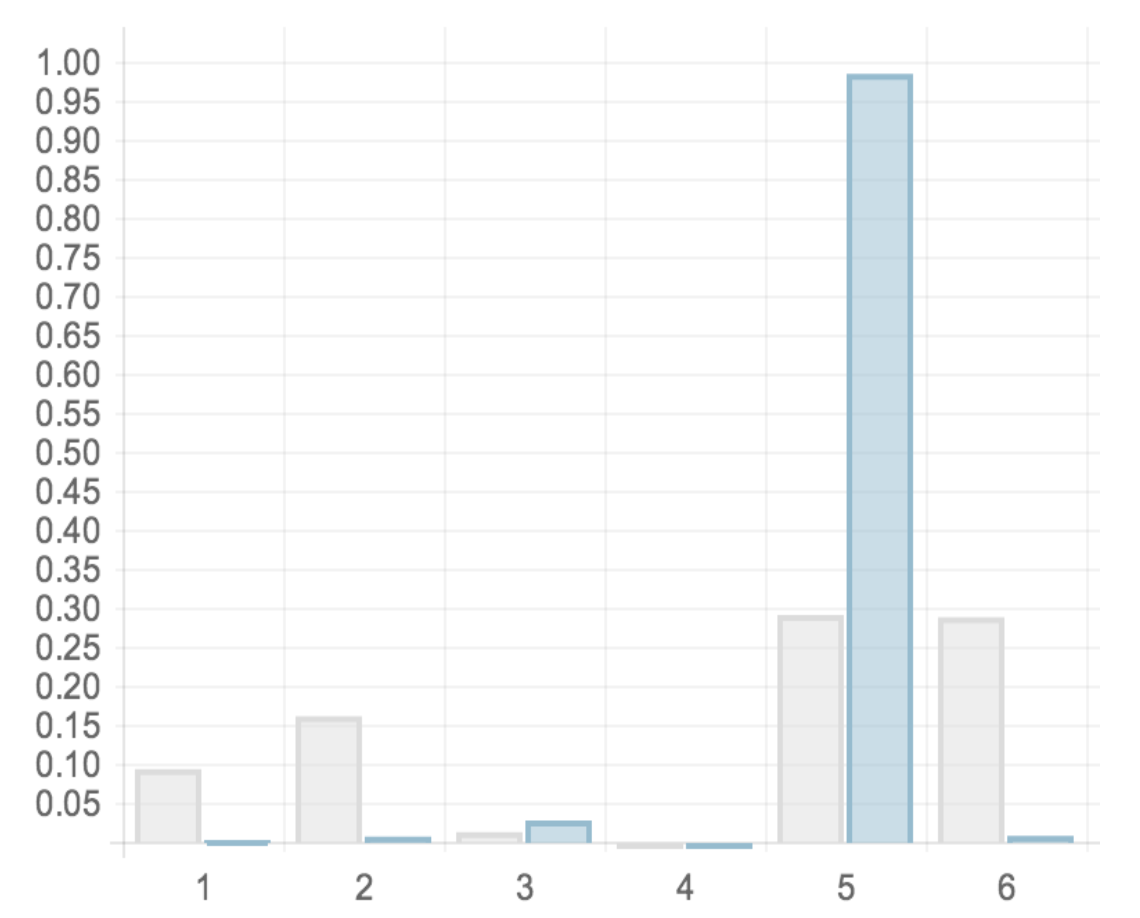
\includegraphics[width=\textwidth]{Figures/clusterings/confluence-post/cluster2-chart}
    \caption{Cluster 2: Users trying out the service alone}
    \label{fig:cluster2-chart}
  \end{subfigure}

  \begin{subfigure}[t]{0.45\textwidth}
    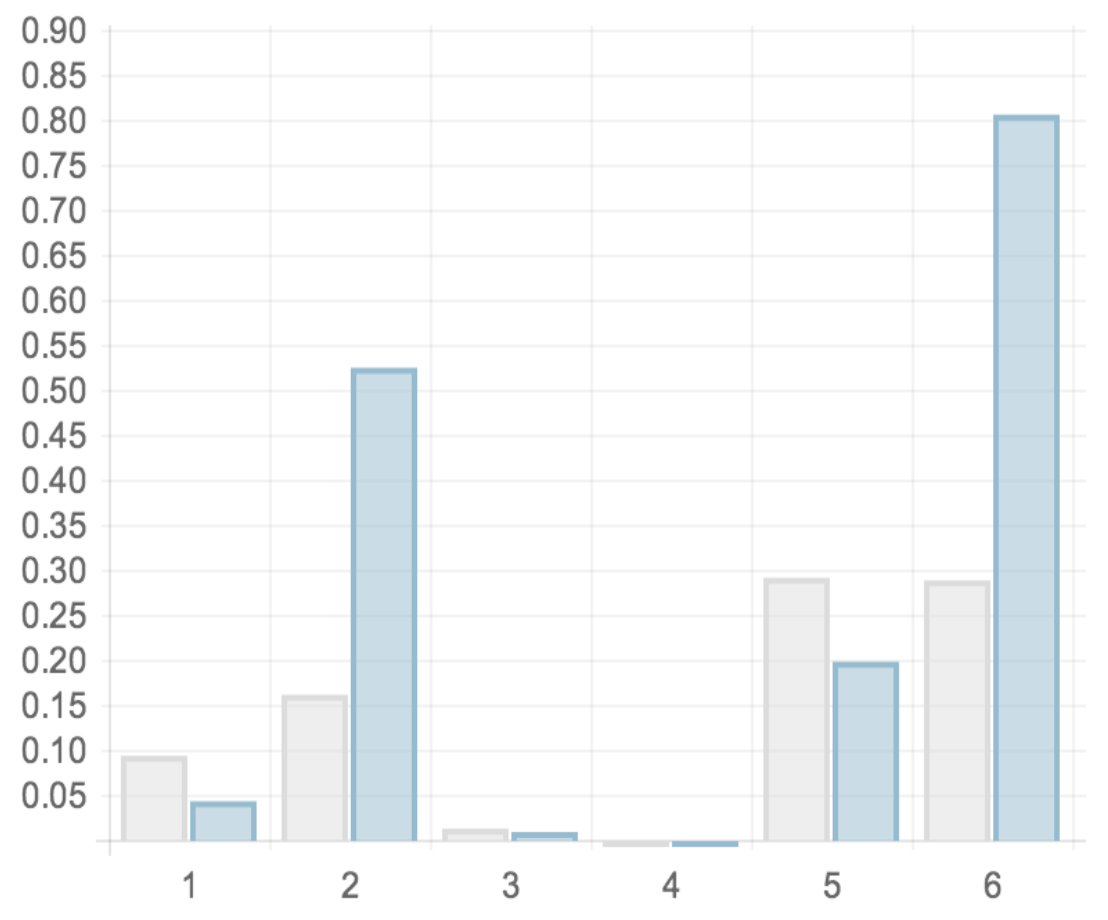
\includegraphics[width=\textwidth]{Figures/clusterings/confluence-post/cluster3-chart}
    \caption{Cluster 3: Simple users with small networks}
    \label{fig:cluster3-chart}
  \end{subfigure}
  \hfill
  \begin{subfigure}[t]{0.45\textwidth}
    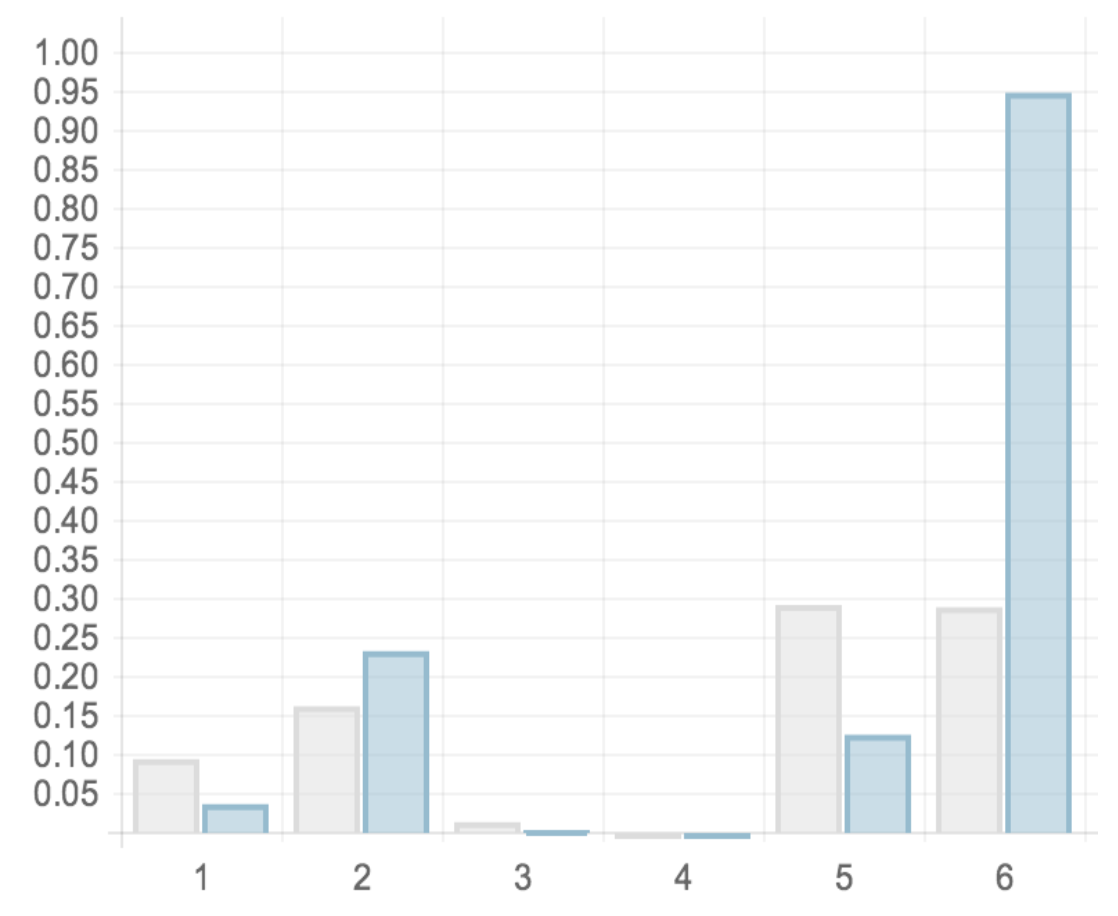
\includegraphics[width=\textwidth]{Figures/clusterings/confluence-post/cluster4-chart}
    \caption{Cluster 4: Simple users with large networks}
    \label{fig:cluster4-chart}
  \end{subfigure}

  \begin{subfigure}[t]{0.45\textwidth}
    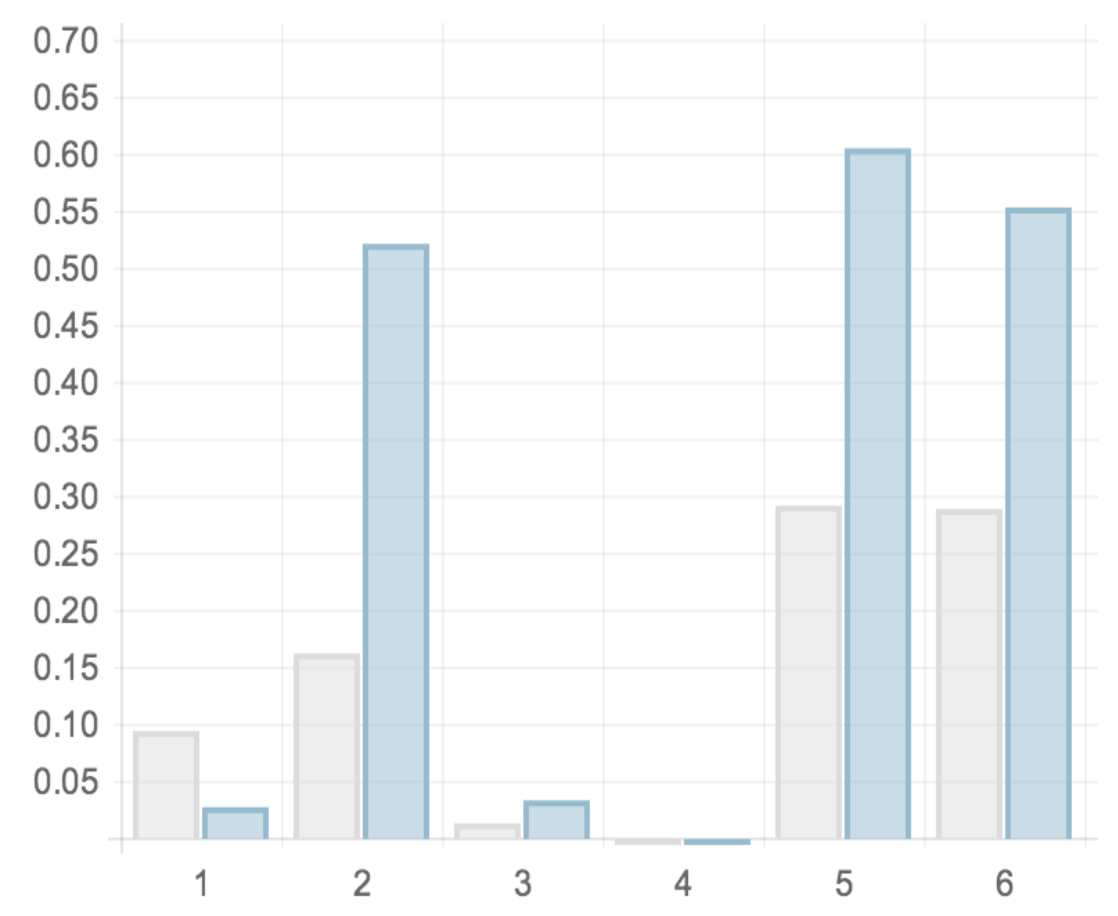
\includegraphics[width=\textwidth]{Figures/clusterings/confluence-post/cluster5-chart}
    \caption{Cluster 5: Incognito users}
    \label{fig:cluster5-chart}
  \end{subfigure}
  \hfill
  \begin{subfigure}[t]{0.45\textwidth}
    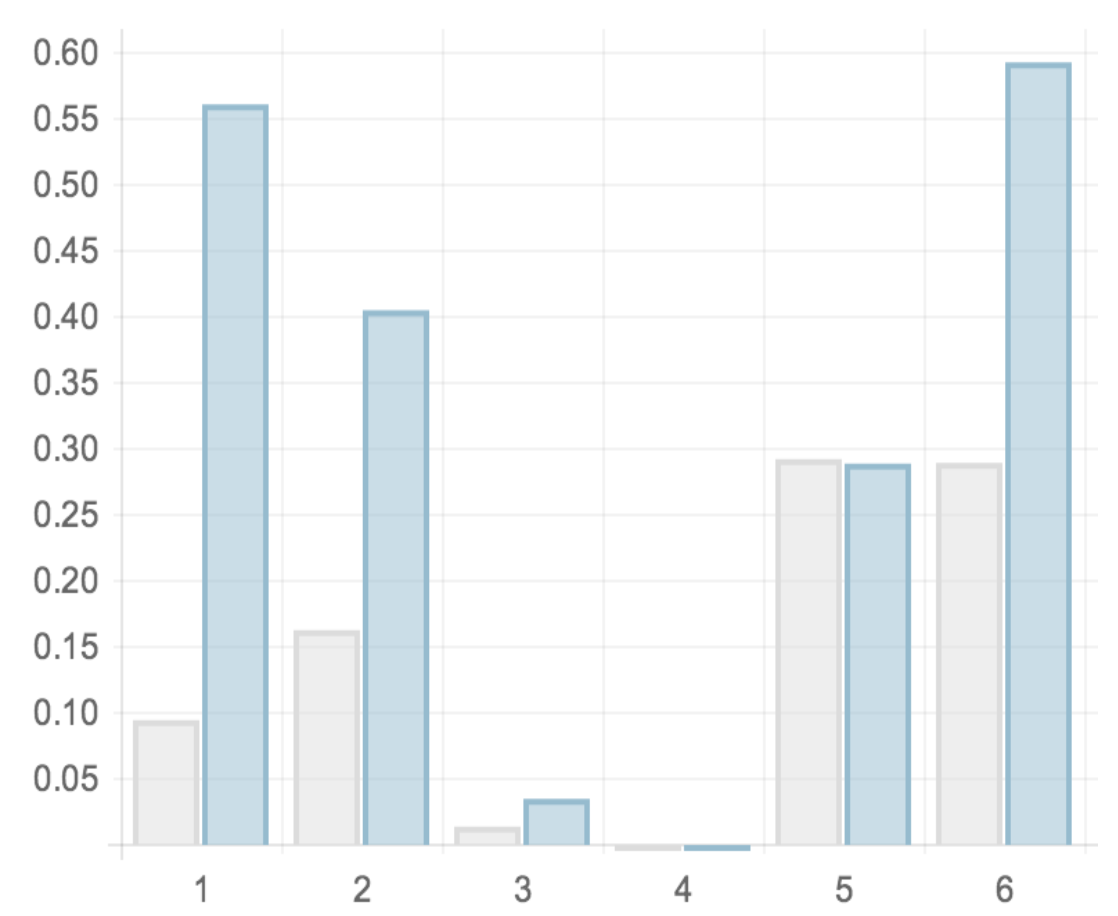
\includegraphics[width=\textwidth]{Figures/clusterings/confluence-post/cluster6-chart}
    \caption{Cluster 6: Chatty, simple users}
    \label{fig:cluster6-chart}
  \end{subfigure}

  \caption{Cluster centers compared to the unweighted average cluster centers. \\ The features plotted are 1) chat messages sent, 2) conversations, 3) rooms claimed, 4) rooms followed, 5) unique rooms used, and 6) conversation network size.}
\end{figure}

\subsubsection{Cluster 1: Front page hits}

The centroid for this cluster is quite simply $\mu_1 = \langle 0, 0, 0, 0, 0, 0 \rangle$.

\begin{persona}
  The user has not tried the actual service -- most likely hitting the front page and either not using a compatible device/browser, or not finding it interesting enough to try out.
\end{persona}

\subsubsection{Cluster 2: Trying out the service alone}

As shown in figure~\ref{fig:cluster2-chart}, the users in this cluster score close to 0 on every feature except the number of rooms used -- most notably, the number of conversations.

\begin{persona}
  The user has tried out the service, but not ever conversed with another user.
\end{persona}

\subsubsection{Cluster 3: Simple users with small networks}

Users in cluster 3 (see figure~\ref{fig:cluster3-chart}) don't use any of the more advanced features of the service, like chatting, claiming or following a room, but on average they have taken part in just over 5 conversations.

\begin{persona}
  A returning user, only utilizing the bare functionality, conversing only with a very limited group of people.
\end{persona}

\subsubsection{Cluster 4: Simple users with large networks}

The users in cluster 4 (see figure~\ref{fig:cluster4-chart}) are very much like the ones in cluster 3, but use the service slightly more, and are part of much larger networks.

\begin{persona}
  A returning user, only utilizing the bare functionality, part of a large group of people using the service.
\end{persona}

\subsubsection{Cluster 5: Incognito users}

To track users over time, cookies are required. Whenever clearing the browser cache, or when browsing in ``incognito mode''\footnote{Browsing without storing any data, including cookies.}, the service will not be able to tie together user sessions. These perceived one-off users should end up in this cluster, close to the pattern shown in figure~\ref{fig:cluster5-chart}.

\begin{persona}
  A user browsing in incognito mode, or who clears the browser cache regularly.
\end{persona}

\subsubsection{Cluster 6: Chatty simple users}

The users of cluster 6 are very much like those in cluster 3, as can be seen in figure~\ref{fig:cluster6-chart}. The significant difference is that they make heavy use of the chat functionality.

\begin{persona}
  A user sharing the characteristics of users in cluster 3, except in making use of the text chat functionality.
\end{persona}

\section{Adapting the user interface} % (fold)
\label{eval:sec:adapting_the_user_interface}

The adaptation component consists of two important steps.

\begin{enumerate}
  \item Determine which type of user (ie. \emph{cluster}) will have the most to gain from having feature $f$ enabled.
  \item Tagging the users with cluster and enabling features for
\end{enumerate}

\subsection{Evaluating the results} % (fold)
\label{eval:sec:evaluating_the_results}

Seeing as the application does not yield any direct and real payoff, we will evaluate the performance of each variation relatively, using some general key metrics. This approach is described in~\cite{Yue2012}.

For appear.in, the most important key metrics are ``time on site'' and ``number of visits in the last $n$ days''. These are combined in providing a relative success metric for each variation.

\emph{@TODO: Verify key metrics.}

% subsection evaluating_the_results (end)


% section adapting_the_interface (end)

\section{Results} % (fold)
\label{eval:sec:results}

\begin{table}
  \begin{tabular}{| lr |  rrr| rrr| rrr| c|}
\hline
 \multicolumn{2}{|l|}{Variations} & \multicolumn{3}{|c|}{off} & \multicolumn{3}{|c|}{on} & \multicolumn{3}{|c|}{total} & \\
\hline
 $C$ & $|C|$ & n & c & \% & n & c & \% & n & c & \% & preferred \\
\hline
1 & 92,762 & 42 & 0 & 0.00 & 43 & 0 & 0.00 & 85 & 0 & 0.00 & off \\
2 &  3,566 & 21 & 9 & 42.86 & 16 & 11 & 68.75 & 37 & 20 & 54.05 & on \\
3 &    607 & 156 & 75 & 48.08 & 152 & 67 & 44.08 & 308 & 142 & 46.10 & off \\
4 &    442 & 151 & 90 & 59.60 & 160 & 113 & 70.62 & 311 & 203 & 65.27 & on \\
5 &    377 & 118 & 106 & 89.83 & 133 & 125 & 93.98 & 251 & 231 & 92.03 & on \\
6 &    584 & 180 & 145 & 80.56 & 165 & 134 & 81.21 & 345 & 279 & 80.87 & on \\
\hline
\end{tabular}

% sizes: [92762, 3566, 607, 442, 377, 584]
% ids: [2135, 2136, 2137, 2138, 2139, 2140]

  \caption{A result.}
  \label{tab:results}
\end{table}

% section results (end)

\section{Discussion} % (fold)
\label{eval:sec:discussion}

% section discussion (end)
